\documentclass{article}

\usepackage[margin=3cm]{geometry}

\geometry{a4paper,left=2cm,right=2cm,top=2.54cm,bottom=2.54cm}
%加這個就可以設定字體
\usepackage{fontspec}
    % 普通文字,行距
        \usepackage[onehalfspacing]{setspace}
    
    % 段落間距  (begin doc 才設定)
        \usepackage{parskip}
%使用xeCJK,其他的還有CJK或是xCJK
    % 中文
    \usepackage{xeCJK}
    \setCJKmainfont[AutoFakeBold=3]{DFKai-SB} %设置中
    \usepackage[fontsize=14pt]{fontsize}
% 首行縮排距離
    \setlength\parindent{28pt}
        % 首行縮排
        \usepackage{indentfirst}

%%%%%%%%%%%%%%%%%%%%%%%%
%%%%    三、圖片
%%%%%%%%%%%%%%%%%%%%%%%%


    %%%%    啟用圖片功能
    \usepackage{graphicx}

    %%%%    設定圖片路徑
    \graphicspath{ {./img/} }

    %%%%    設定圖片定位
    \usepackage{float}

    %%%%    把Figure變成"圖"
    \renewcommand{\figurename}{Fig}

%%%%%%%%%%%%%%%%%%%%%%%%
%%%%%%%              end

% 目錄顯示層次
    \setcounter{tocdepth}{2}
% 計算
\usepackage{enumitem}

%設定英文字型,不設的話就會使用預設的字型
\setmainfont{Times New Roman}

\usepackage{fontspec}
\usepackage{titlesec}
\usepackage{graphicx}
\usepackage{physics}
\usepackage{amsmath}
\usepackage{mathtools}
\usepackage{setspace}
\usepackage{subfigure} %所需宏包

\usepackage[hidelinks]{hyperref}
 \usepackage{titlesec}
    % 定义section格式,包括中文数字
   
    \usepackage{zhnumber}
\titleformat{\section}
  {\fontsize{18pt}{15}\bfseries}
  {\selectfont\thesection.}
  {0.5em}
  {}

\usepackage{fancyhdr}
\pagestyle{fancy}

\usepackage{color, xcolor}

\usepackage{algorithm}
\usepackage{algpseudocode}


% New definitions
\algnewcommand\algorithmicswitch{\textbf{switch}}
\algnewcommand\algorithmiccase{\textbf{case}}
\algnewcommand\algorithmicassert{\texttt{assert}}
\algnewcommand\Assert[1]{\State \algorithmicassert(#1)}%
% New "environments"
\algdef{SE}[SWITCH]{Switch}{EndSwitch}[1]{\algorithmicswitch\ #1\ \algorithmicdo}{\algorithmicend\ \algorithmicswitch}%
\algdef{SE}[CASE]{Case}{EndCase}[1]{\algorithmiccase\ #1}{\algorithmicend\ \algorithmiccase}%
\algtext*{EndSwitch}%
\algtext*{EndCase}%

\usepackage{newfloat}
\DeclareFloatingEnvironment[
  fileext = lol ,
  listname = {List Of Listings} ,
  name = Listing
]{listing}

\makeatletter
\newenvironment{breakablealgorithm}
  {% \begin{breakablealgorithm}
    \footnotesize
   \begin{center}
     \refstepcounter{algorithm}% New algorithm
     \hrule height.8pt depth0pt \kern2pt% \@fs@pre for \@fs@ruled
     \renewcommand{\caption}[2][\relax]{% Make a new \caption
       {\raggedright\textbf{\ALG@name~\thealgorithm} ##2\par}%
       \ifx\relax##1\relax % #1 is \relax
         \addcontentsline{loa}{algorithm}{\protect\numberline{\thealgorithm}##2}%
       \else % #1 is not \relax
         \addcontentsline{loa}{algorithm}{\protect\numberline{\thealgorithm}##1}%
       \fi
       \kern2pt\hrule\kern2pt
     }
  }{% \end{breakablealgorithm}
     \kern2pt\hrule\relax% \@fs@post for \@fs@ruled
   \end{center}
  }
\makeatother

\usepackage{pdfpages}
\algnewcommand\And{\textbf{and}}
\algnewcommand\Or{\textbf{or}}

\usepackage{amsmath}

\newcommand\mycommfont[1]{\footnotesize\ttfamily\textcolor{mygreen}{#1}}

\usepackage{tikz, ifthen}
\usetikzlibrary{calc,shapes, positioning,chains,arrows}

\usepackage{everyshi}  % 用于在每一页应用浮水印


% 畫底線
\usepackage{ulem}


\definecolor{myblue}{HTML}{6B73D5}
\definecolor{myred}{HTML}{C00000}
\definecolor{myyellow}{HTML}{FFDB57}

\usepackage[hidelinks]{hyperref}
\hypersetup{urlcolor=myblue, % url
citecolor=black, % citation
linkcolor=black, % table of contents, inner color
colorlinks=true, }
\usepackage{enumitem}

\usepackage{listings}

\definecolor{Blue}{rgb}{0,0,1}
\definecolor{Green}{rgb}{0,0.5,0}
\definecolor{Red}{rgb}{0.64,0.08,0.08}


\lstset{
    captionpos=t,                       % 讓Caption在Bottom的位置
    numbers=left,                       % 程式碼行號
    frame=single,
    showstringspaces=false,             % "不"標註空格
    escapeinside={(*@}{@*)},            % 脫逃字元
    commentstyle=\color{Green},         % Comment顏色
    keywordstyle=\color{Blue},          % Keyword顏色
    stringstyle=\color{Red},            % String顏色
    basicstyle=\ttfamily\scriptsize,         % 字型
    breaklines = true,
}


\begin{document}



\thispagestyle{empty}

\begin{center}
        \vspace*{3cm} %垂直距離
        {\Huge\bf
            \underline{CAD for VLSI Design }\\}%\uppercase\expandafter{\romannumeral 1}}
        \vspace{3cm}
        {\bf\huge Project Assignment 3\\}
        \vspace{0.5cm}
        {\bf\fontsize{23pt}{20}\selectfont Analog Placement\\}
        \vspace{4cm}
        {\fontsize{23pt}{26pt} \selectfont Instructor: Andy, Yu-Guang Chen  Ph.D.\\}
        {\fontsize{20pt}{26pt} \selectfont TA: 曹寓恆\\}
        \vspace{2cm}
        \fontsize{22pt}{25pt}\selectfont
        Department/Class: Electrical Engineering 4A\\
        \vspace*{1em}
        Name: {\bf 陳緯亭}\\
        \vspace*{1em}
        Student ID Number: {\bf 109501201}\\
\vspace{2cm}
\end{center}
\newpage


\tableofcontents
\listoflistings


\thispagestyle{empty}
\newpage


 \setcounter{page}{1}

 \lhead{109501201\ 陳緯亭}

% --------------------------------------------------------


\section{How I compile and execute the program}

\begin{figure}[H]
  \centering
  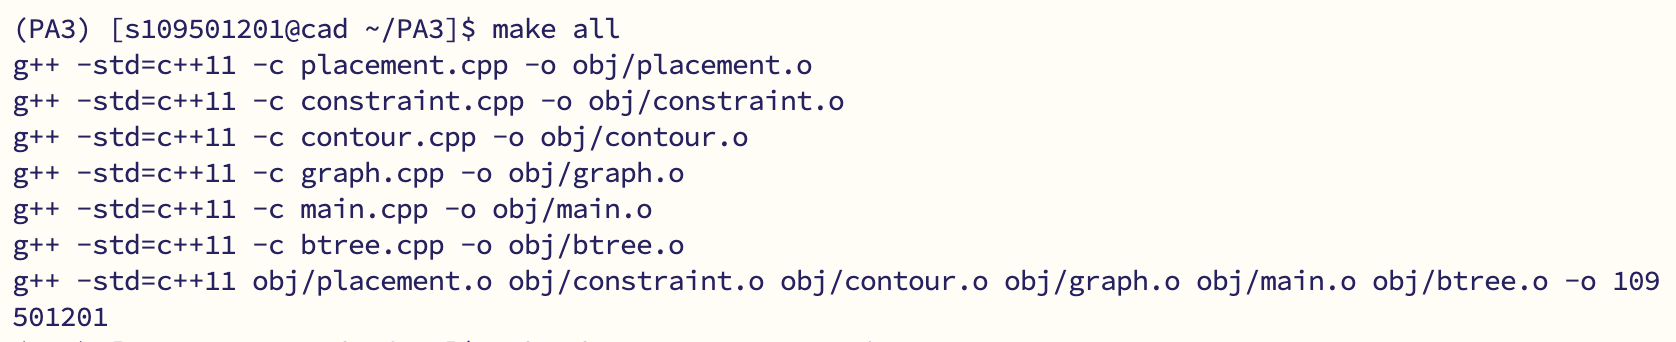
\includegraphics[width=\linewidth]{./img/2024-05-26-19-11-41.png}
  \caption{Compile my source code and generate the corresponding objects}
  \label{g++}
\end{figure}

\vspace*{-1em}

\begin{figure}[H]
  \centering
  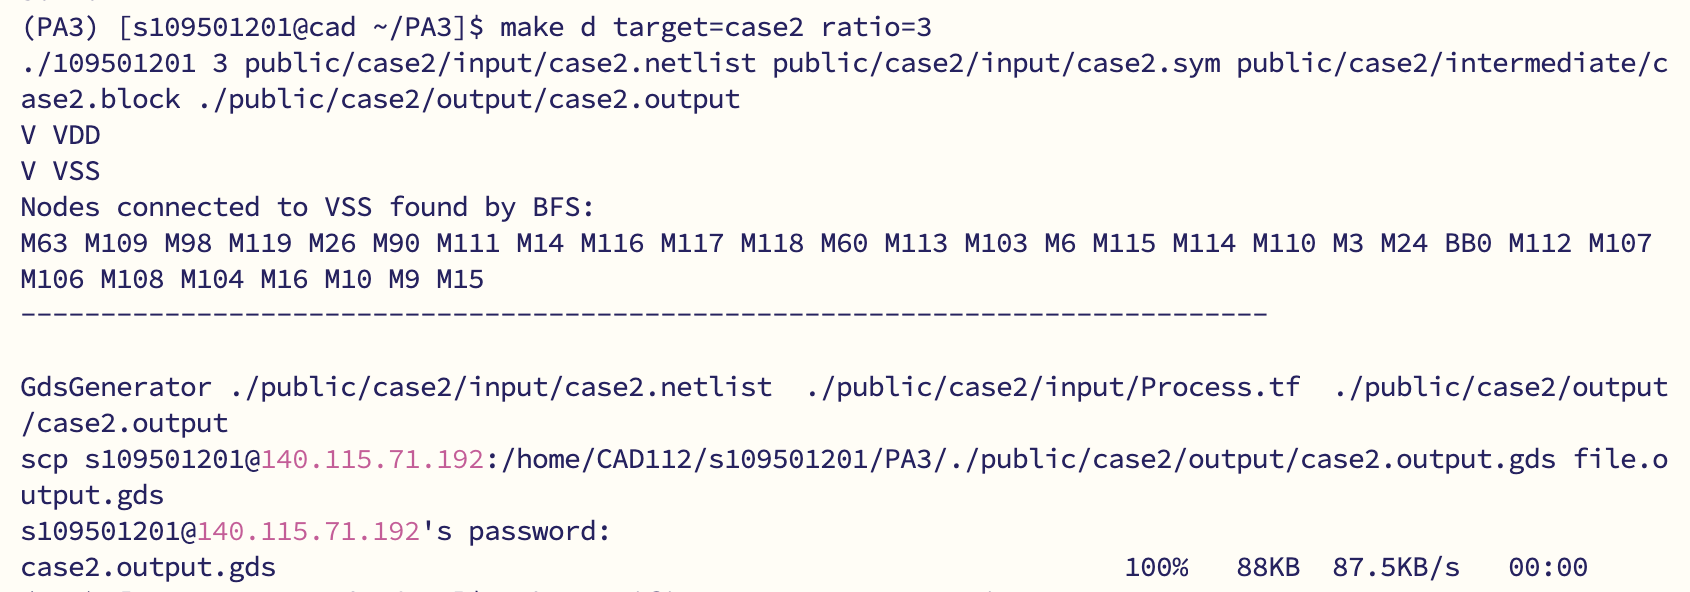
\includegraphics[width=\linewidth]{./img/2024-05-26-19-12-58.png}
  \caption{Execute my analog placer and then download GDSII File for visualization purposes}
  \label{gdsii}
\end{figure}


\begin{figure}[H]
    \centering
    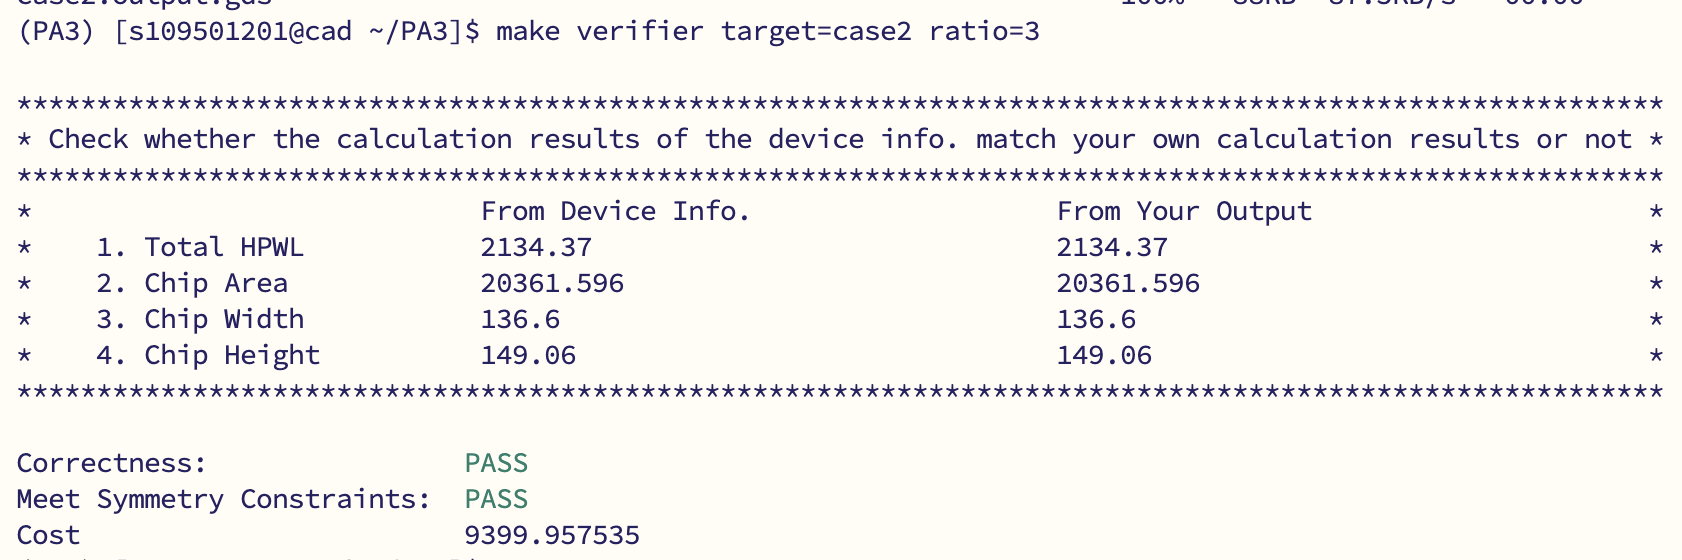
\includegraphics[width=\linewidth]{./img/2024-05-26-19-15-10.png}
    \caption{Run verifier}
    \label{verifier}
  \end{figure}

\pagebreak

\section{Pseudo Code}

\begin{breakablealgorithm}
    \caption{Build a Tree}
    \begin{algorithmic}[1]
      \Function{buildATree}{root, left, recurse, max\_x, max\_y, map, path}
      \If{$root = \text{nullptr}$}
        \State \Return
      \EndIf
      \State $w \gets$  root width, $h \gets$  root height
      \State $axis \gets root \rightarrow axis$
      
      \If{$root \rightarrow parent = \text{nullptr}$} \Comment{Root node}
        \State $root \gets $ Initialize
      \Else
        \State $pw \gets $ parent width, $ph \gets $parent height
        \If{$root$ is self-symmetry module}
          \State $root\ x \gets parent\ center\_x$
        \Else
          \State $root\ x \gets parent\ max\_x$
        \EndIf
  
        \If{$root$ is in the symmetry file}
          \If{$root$ is self-symmetry module}
            \State $root\ x \gets root\ x - w / 2$
          \Else
            \State $root\ x \gets root\ x - w$
          \EndIf
        \ElsIf{$left$}
          \State $root\ x \gets root\ x + parent\ axis + root\ axis$
          \If{$root$ is self-symmetry module}
            \State $root\ x \gets root\ x - w / 2$
          \Else
            \State $root\ x  \gets root\ x - w$
          \EndIf
        \Else
          \State $root\ x \gets root\ x - parent\ axis + root\ axis$
          \If{$root$ is self-symmetry module}
            \State $root\ x \gets root\ x - w / 2$
          \Else
            \State $root\ x \gets root\ x - w$
          \EndIf
        \EndIf
  
        \State $root\ center\_x \gets root\ x + w / 2$
        \State $root\ max\_x \gets root\ x + w$
  
        \If{$root$ is self-symmetry module}
          \State $y \gets $ from checking contour
        \Else
          \State $y \gets$ from checking contour
        \EndIf
  
        \State $root\ y \gets y$
        \State $root\ max\_y \gets y + h$
        \State $root\ center\_y \gets y + h / 2$
      \EndIf
  
      \If{$root\ max\_x > max\_x$}
        \State $max\_x \gets root\ max\_x$
      \EndIf
      \If{$root\ max\_y > max\_y$}
        \State $max\_y \gets root\ max\_y$
      \EndIf
  
      \State  refresh contour
      \If{$root \neq \text{nullptr}$}
        \If{$root$ is self-symmetry module}
          \State create another MOS in symmetry pair location
        \EndIf
      \EndIf
  
      \If{$recurse$}
        recurse
      \EndIf
      \EndFunction
    \end{algorithmic}
  \end{breakablealgorithm}

  \begin{figure}[H]
    \centering
    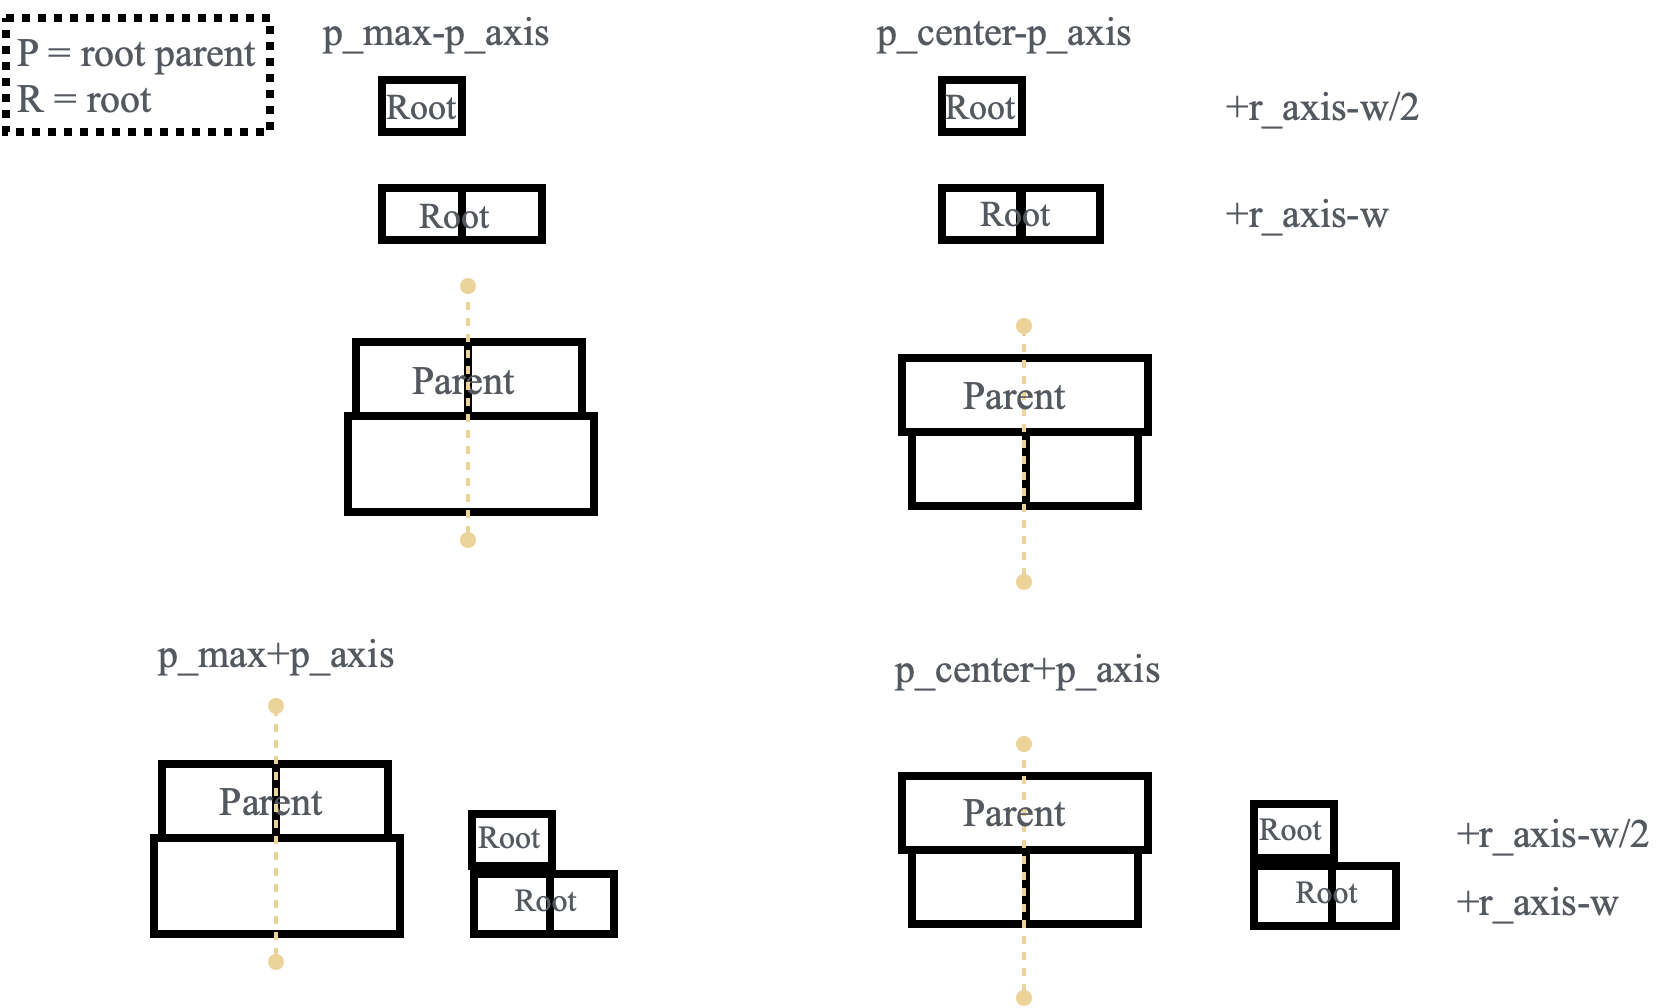
\includegraphics[width=0.65\linewidth]{./img/2024-05-26-21-07-40.png}
    \caption{Find block ocation}
\end{figure}


\subsection{The degree of completion of the assignment: \textcolor{red}{Perturbation Not Yet Complete}}

\section{Algorithms and data structures}

There are four structures in my programme, InBlock, InSym, TreeNode and Contour. InBlock is for collecting input data from the .block file. InSym is for storing the information in a symmetry constraint file. TreeNode is for constructing the b* tree. And Contour is to record the y-contour to prevent block from overlapping.

\lstinputlisting[caption={The data structure}, label={struct}, language={c++}, firstnumber=last]{./Structure.cpp}


\begin{figure}[H]
    \centering
    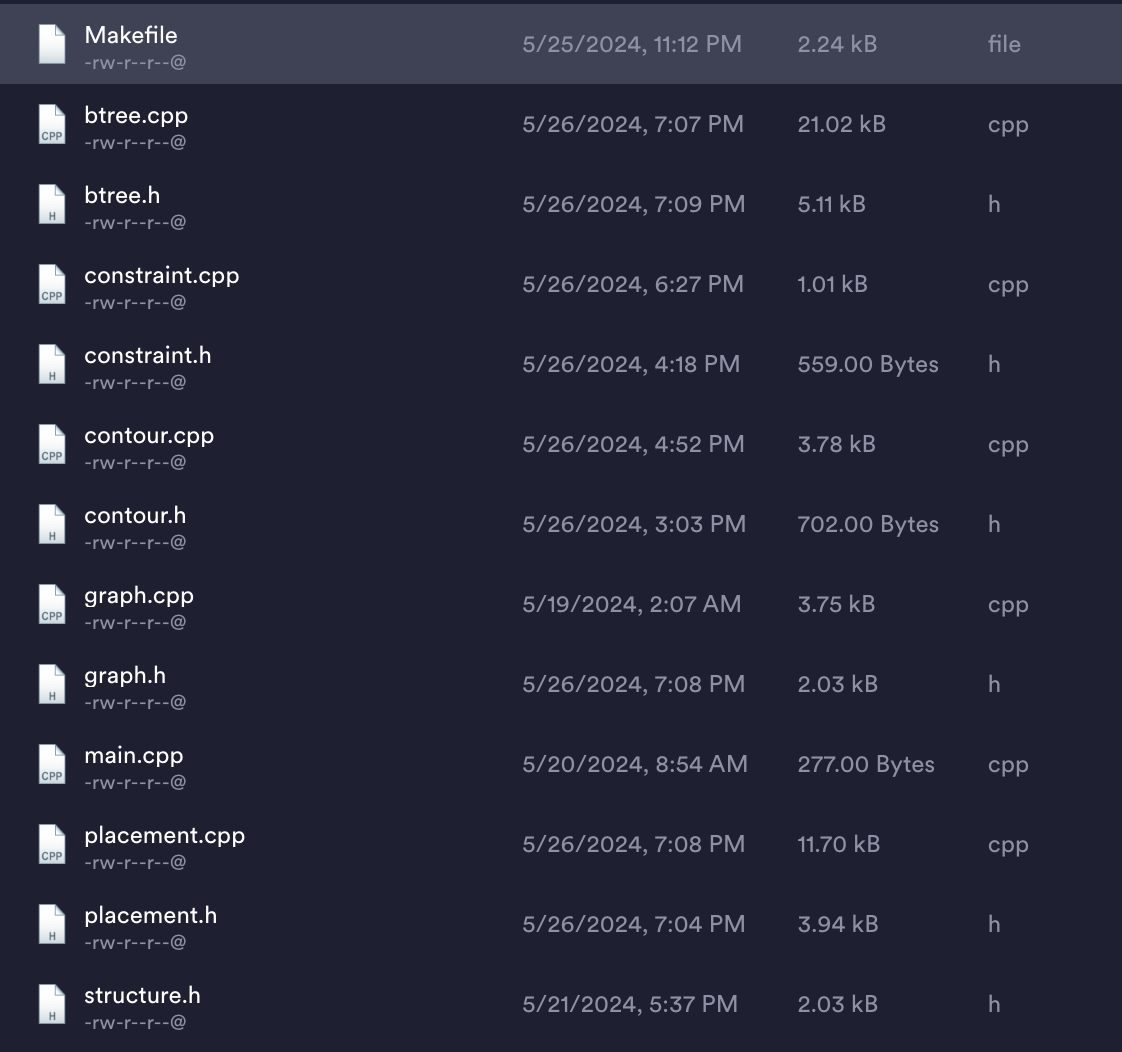
\includegraphics[width=0.8\linewidth]{./img/2024-05-26-19-57-06.png}
    \caption{Source code}
    \label{source code}
  \end{figure}
  
  \begin{figure}[H]
    \centering
    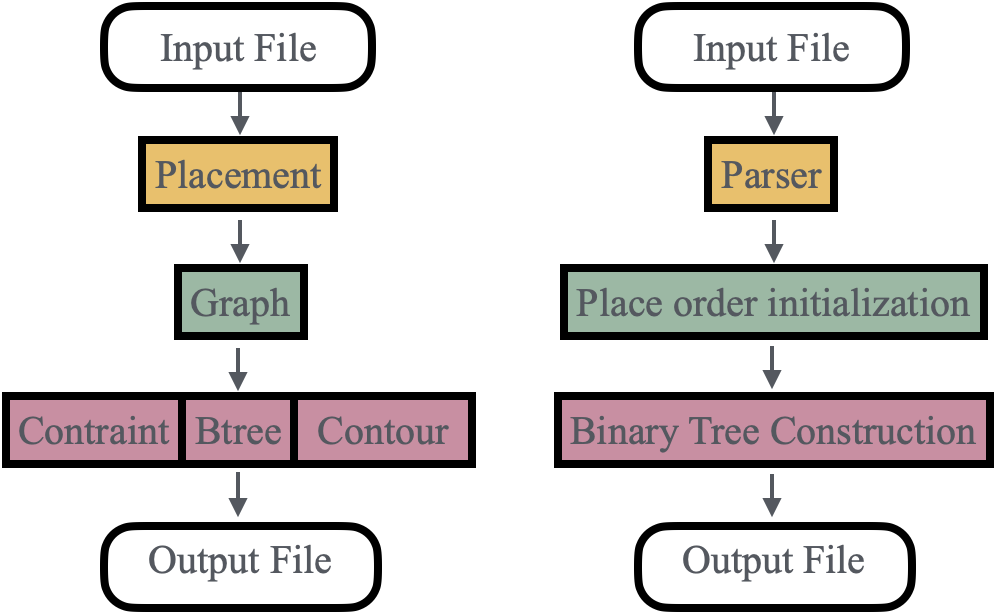
\includegraphics[width=0.5\linewidth]{./img/2024-05-26-20-41-36.png}
    \caption{Source File and its functions}
    \label{file order}
  \end{figure}


  The program is constructed using six .cpp files and six .h files. The placement.cpp file serves as a parser for both the input and output files. The graph.cpp file is responsible for arranging the blocks that are placed in the first instance. The btree.cpp file is used to construct a b*-tree and employs a pre-order traversal to traverse all the data. The constraint.cpp file ensures that the aspect ratio limitations are met, thus preventing the blocks from becoming excessively long. Finally, the contour.cpp file is responsible for processing the y location in order to place the blocks.

\section{Perturbation strategy and operations}

Using Simulated Annealing to pick the new TreeNode according to cost function in constraint.cpp. This is not completed. Therefore, the refresh TreeNode answers are wrong.

\lstinputlisting[caption={The Simulated Annealing}, label={sa}, language={c++}, firstnumber=last]{./SA.cpp}

\section{Cost function and how to determine to next state}

The cost function should come in the area, minimize half-perimeter wire length, my aspect ratio and the expected ratio from input. It should be used in the Simulated Annealing.

\lstinputlisting[caption={Cost function}, label={Cost function}, language={c++}, firstnumber=last]{./cost.cpp}

The aspect ratio is $max\left(\dfrac{w}{h}, \dfrac{h}{w}\right)$.

\lstinputlisting[caption={Aspect ratio}, label={Aspect ratio}, language={c++}, firstnumber=last]{./ratio.cpp}

\pagebreak
% ------------------------------
\section{The hardness of this assignment / I overcome it}

\begin{enumerate}
    \item Contour can't not be refresh in the correct y.\\
    Ans: The contour value $(x_1, x_2, y_1)$ and the check scale $(x_3, x_4, y_2)$ are set, and if $x_3 = x_2$, then $y_2$ would be $y_1$. I didn't expect that. So I give it a little bias ($x_1=x_1+0.0001$) to solve this problem.

    \item How to find the axis in self-symmetry module and symmetry pair?\\
    Ans: I find that it can be solved by using recursion.
    \item How to place the block and mos?\\
It is necessary to consider whether the parent is a symmetry pair or self-symmetric, as well as whether the object itself is a symmetry pair or self-symmetric.
    

\end{enumerate}

% ------------------------------

\section{Suggestions}

No.

\end{document}